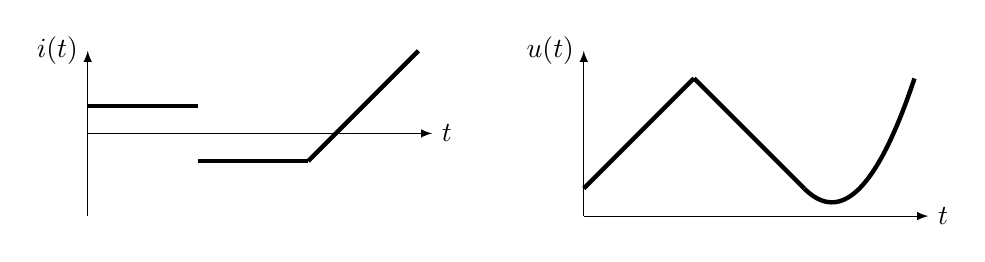
\begin{tikzpicture}[
	scale=.7,
	trait1/.style={thick,smooth,samples=50,draw=\JRLorange},
	trait2/.style={thick,smooth,samples=50,draw=\JRLgreen},
]
\begin{scope}
\shorthandoff{:!}
\draw[-latex] (0,0) -- (6.25,0) node[right]{$t$};
\draw[-latex] (0,-1.5) -- (0,1.5) node[left]{$i(t)$};
\draw[trait1,domain=0:2, ultra thick] plot (\x,0.5);
\draw[trait1,domain=2:4, ultra thick] plot (\x,-0.5);
\draw[trait1,domain=4:6, ultra thick] plot (\x,{\x-4.5});
\end{scope}
%%%%%%%%%%%%%%%%%%%%%%
\begin{scope}[shift={(9,-1.5)}]
\draw[-latex] (0,0) -- (6.25,0) node[right]{$t$};
\draw[-latex] (0,0) -- (0,3) node[left]{$u(t)$};
\draw[trait2,domain=0:2, ultra thick] plot (\x,0.5+\x);
\draw[trait2,domain=2:4, ultra thick] plot (\x,4.5-\x);
\draw[trait2,domain=4:6, ultra thick] plot (\x,{\x^2-9*\x+20.5});
\end{scope}

\end{tikzpicture}